\noindent \texttt{V: 24-03-2023 23:16:00}

\section*{Experimento: - Máquinas Eletrostáticas - Gerador Van De Graaff}

\section*{Teoria}
\subsection*{Introdução}

\begin{wrapfigure}{R}{0.3\textwidth}
\centering
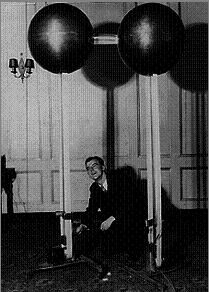
\includegraphics[width=0.7\linewidth]{img/rj-vandegraaff.png} 
	\caption{Robert J. Van de Graaff e uma das primeiras versões do Gerador Van de Graaff \textit{Fonte: http://www.cmm.gov.mo}.}
	\label{fig:robert-j-vgraaff}
\end{wrapfigure}
Por volta de 1930, o engenheiro estado-unidense Robert Jeminson Van de Graaff inventou uma 
máquina capaz de demonstrar de forma visível a ação da eletricidade a partir da transferência das 
cargas elétricas de um corpo eletrizado para outro. Em sua homenagem, esse aparelho foi batizado
de Gerador de Van de Graaff. Seus princípios ainda são utilizados atualmente, a máquina atua na 
física nuclear, em versões mais potentes, para produzir tensões muito elevadas em aceleradores de 
partículas, assim como na medicina e na indústria de alta tecnologia.

\noindent Essa máquina será fundamental para atingir o objetivo do experimento que será realizado em 
laboratório. Sob instruções do Professor, a turma de Física Experimental III
utilizará o Gerador de Van de Graaff para executar três procedimentos em laboratório e 
verificar as manifestações da força elétrica e o comportamento das cargas estáticas submetidas à 
situações de transferência de cargas entre dois corpos, bem como para analisar a disposição dessas 
cargas de acordo com o formato de cada corpo e seus efeitos resultantes.

\subsection*{Fundamentos da Eletrostática e Gerador Van De Graaff}
Os fundamentos básicos da eletrostática regem o funcionamento do Gerador de Van de Graaff, 
sendo eles: o Princípio da atração e repulsão, responsável por demonstrar que cargas de mesmo 
sinal tendem a se repelir e cargas de sinais contrários tendem a se atrair. O Princípio da conservação 
de cargas, o qual define que a quantidade total de cargas de um sistema é sempre constante. E os 
tipos de eletrização (Atrito, Contato e Indução) que definem como acontece a transferência das 
cargas. De maneira geral, pode-se dizer o gerador auto-excitado funciona de acordo com os princípios do \textbf{efeito tribolelétrico}, se referindo ao fenômeno que ocorre quando dois materiais de composição diferentes estão bem juntos e então são puxados de maneira que se separem num curto intervalo de tempo.

O gerador de Van de Graaff funciona através da movimentação de uma correia que é eletrizada por 
atrito na parte inferior do aparelho. Ao atingir a parte superior, as cargas elétricas que surgiram com o processo de eletrização por Atrito, são transferidas para a superfície interna do metal, sendo então 
distribuídas para toda a superfície da esfera metálica, ficando carregada de cargas elétricas. Se durante o funcionamento do gerador aproximarmos o dedo ou um objeto de metal perceberemos leves descargas elétricas que ocorrem em razão da diferença de potencial. 
De maneira geral, esse gerador é composto por:

\begin{itemize}
    \item  Um motor; 
    \item  Dois cilindros (um condutor e outro isolante); 
    \item  Um conjunto de correias; 
    \item  Um conjunto de escovas; 
    \item  Um terminal de saída, que na maioria das vezes é uma grande esfera metálica ou recoberta por um material condutor.
\end{itemize}



\section*{Prática}
\section{Objetivos}
\begin{itemize}
    \item[i] Verificar comportamento de cargas estáticas e as manifestações da Força Elétrica;
    \item[ii] Faça a revisão bibliográfica sobre o assunto: "Fundamentos da eletrostática e do Gerador de Van De Graaff";
    \item[iIi] Faça algumas imagens do experimento.
\end{itemize}

\section{Material Utilizado}
\begin{itemize}
    \item Gerador Van De Graaff
    \item Eletroscópio
    \item Condutores Pontiagudos (Lança, Torniquete)
    \item Vela
    \item Lâmpadas de Gazes diversos (Ionização e DDP)
    \item Diversos fios condutores e acessórios
\end{itemize}
\par 
\noindent oi

\section{Procedimento experimental}
Realizar três experimentos para observar o comportamento das cargas elétricas, sendo eles:

\begin{itemize}
    \item  Força Elétrica - Eletroscópio
    \item  Poder das Pontas - “Para-raios”
    \item  Vento Iônico
\end{itemize}

\subsection{Força elétrica – Eletroscópio:}

\subsubsection{FUNÇÃO:}

\noindent Esse experimento teve a função de verificar se um corpo está ou não eletrizado, assim como observar a intensidade da sua eletrização

\subsubsection{MATERIAIS UTILIZADOS:} 
\begin{itemize}
    \item[a)] Gerador de Van de Graaff
    \item[b)] Material isolante
    \item[c)] Fios condutores
    \item[d)] Eletroscópio
    \item[e)] Corpo condutor que será eletrizado
\end{itemize}

\subsubsection{PROCEDIMENTO:} 
Ligou-se o Gerador de Van de Graaff na corrente elétrica, a qual fez a correia movimentar-se entre as escovas, eletrizando-a por atrito. As cargas negativas chegaram até a esfera de alumínio por contato.

\noindent Com o gerador eletrizado, aproximou-se uma outra esfera condutora, a qual teve suas cargas separadas por Indução. Após isso, ligou-se a parte positiva da esfera na terra para descarregar as cargas e o corpo também ficar eletrizado negativamente
Sob essas condições, foi possível observar a repulsão das cargas nas extremidades do eletroscópio, quando aproximado de algum dos corpos. Informando-nos que o corpo estava eletrizado.

\subsection{Poder das pontas – “Para-raios”}

\subsubsection{FUNÇÃO:}
Esse experimento teve a função de verificar a distribuição das cargas elétricas em um corpo que 
possui extremidades pontiagudas
\subsubsection{MATERIAIS UTILIZADOS: }
\begin{itemize}
    \item[a)] Gerador de Van de Graaff
    \item[a)] Fios condutores
    \item[a)] Lança pontiaguda
\end{itemize}

\subsubsection{PROCEDIMENTO:}
Antes de ligar o Gerador de Van de Graaff na corrente elétrica, posicionou-se a lança pontiaguda no topo da esfera metálica.

\noindent Assim que o Gerador começou a funcionar, percebeu-se que não houve acúmulo considerável de cargas na superfície da esfera oca, em comparação com os procedimentos anteriores. Em contrapartida, havia grandes concentrações de carga ao redor da lança pontiaguda. Isso deve-se ao princípio do “Poder das Pontas”, que define que as cargas elétricas de um corpo se concentram nas regiões mais pontiagudas, fazendo com que o campo elétrico nas vizinhanças 
dessas pontas atinja determinado valor, ionizando o ar em sua volta, tornando-o condutor. Esse princípio é utilizado nos para-raios, fazendo com que a nuvem eletrizada descarregue suas cargas nas pontas do para-raio. Como o para-raio está ligado a terra, as cargas elétricas recebidas são transferidas ao solo sem nenhum problema. 

\subsection{Vento Iônico}
\subsubsection{FUNÇÃO:}
Esse experimento teve a função de observar a repulsão das cargas elétricas gerada pela ionização 
do ar.
\subsubsection{MATERIAIS UTILIZADOS: }
\begin{itemize}
    \item[a)] Gerador de Van de Graaff
    \item[a)] Fios condutores
    \item[a)] Lança pontiaguda
    \item[a)] Torniquete com 4 pontas em forma de “Z”
    \end{itemize}
    
\subsubsection{PROCEDIMENTO: }
Antes de ligar o Gerador de Van de Graaff na corrente elétrica, posicionou-se a lança pontiaguda no topo 
da esfera metálica com o torniquete conectado à ponta da lança pontiaguda. 
Quando o gerador for ligado na corrente elétrica, deve se observar que o torniquete começará a girar. 
Esse efeito deve-se à ionização do ar nas pontas do torniquete, a qual concentrou as cargas 
devido ao “Poder das pontas” e gerou repulsão dos íons de mesmo sinal, determinando a rotação 
acelerada nas pontas. 


\begin{thebibliography}{9}

\bibitem{jeewett11}
  JEWETT JR, J.W., SERWAY, R. A. 
  \emph{Física para cientistas e engenheiros: Eletricidade e magnetismo},
  CENGANGE Learning,
  São Paulo:
  2011

\bibitem{halliday3}
David Halliday, Robert Resnick, Jearl Walker; \emph{F Fundamentos de Física, Volume 3}, 8ª edição, São Paulo 2010. 
 
\bibitem{juraitis}
JURAITIS, K. R.; DOMICIANO, J. B.; \emph{Capítulo 1 - O Laboratório de Física - Introdução ao Laboratório de Física Experimental}, Londrina, PR, 2009

\bibitem{coeufrj}
COE UFRJ 
\emph{Máquinas Eletrostáticas}, \\ \url{www.coe.ufrj.br/~acmq/eletrostatica.html} -  - Acesso em 23/03/2023

\bibitem{jifufrgs}
IF UFRGS - Instituto de Física - UFRGS
\emph{Circuitos Elétricos}, \\ \url{www.if.ufrgs.br/tex/fis142/mod07/m\_s02.html} - Acesso em 01/05/2017

\bibitem{ifscusp}
IFSC USP
\emph{Gerador eletrostático Van De Graaff}
\\ \url{www.ifsc.usp.br/~strontium/Teaching/Material2010-2\%20FFI0106\%20LabFisicaIII/App01b\%20Eletrostatica.pdf} - Acesso em 24/03/2023.

\bibitem{yumpu}
Projeto para Feira do Saber \emph{Tema: Gerador eletrostático de Van dde Graaff} - 
\\ \url{https://www.yumpu.com/pt/document/read/12806191/gerador-eletrostatico-de-van-de-graaffpdf-colegio-decisao} - Acesso em 25/03/2023.
  
\end{thebibliography}
